\section{Details of Message-Passing Network}
\label{sec:tetris-message-passing}


\begin{algorithm}[h]
\caption{\textsc{LearnableTensorProduct}}
\label{alg:learnable-tp}
\begin{algorithmic}

\Require Tensor Product $\otimes$, Number of Channels $C$ (for Gaunt tensor product).
\Procedure{LearnableTP}{$\x_1, \x_2$}
    \If{$\otimes = \cgtp$}
    \State \Return $\textsc{Linear}(\x_1 \cgtp \x_2)$
    \EndIf
    \If{$\otimes = \gtp$}
    \For{$i = 1, 2, \ldots, C$}
    \Let{$\x_1^{(i)}$}{
        $\textsc{Linear}_1^{(i)}(\x_1)$
    }
    \Let{$\x_2^{(i)}$}{
        $\textsc{Linear}_2^{(i)}(\x_2)$
    }
    \Let{$\x_o^{(i)}$}{
        $\textsc{Linear}_o^{(i)}(\x_1^{(i)} \gtp \x_2^{(i)})$
    }
    \EndFor
    \State \Return 
    $
    \textsc{Concatenate}(\{
    \x_o^{(i)} \ | \ i \in \{1, 2, \ldots, C\} \})$
    \EndIf
\EndProcedure
\State \Return LearnableTP
\end{algorithmic}
\end{algorithm}

\begin{algorithm}[h]
\caption{Operation of our Message Passing Neural Network}
\label{alg:mpnn}
\begin{algorithmic}
\Require Graph $G$, Message Passing Iterations $T$, Cutoff $d_{\text{max}}$, Spherical Harmonic Degree $\ell$, Tensor Product $\otimes$
\State Compute neighbor lists for each node in $G$:
$$(u, v) \in E \iff \norm{\mathbf{r}_u - \mathbf{r}_v} \leq d_{\text{max}}$$
\State Create \textsc{LearnableTensorProduct} from $\otimes$.
\For{$v \in V$}:
\Let{$h_v^{(0)}$}{$[1]$}
\EndFor
\For{$t = 1, 2, \ldots, T$}:
\For{$v \in V$}:
\Let{$h_v^{(t)}$}{$\frac{1}{|\gN(v)|}\sum_{u \in \gN(v)} 
\textsc{MLP}(\norm{\mathbf{r}_u - \mathbf{r}_v}) \times \textsc{LearnableTensorProduct}(h_u^{(t - 1)}, Y_\ell(\mathbf{r}_u - \mathbf{r}_v))$}
\Let{$h_v^{(t)}$}{$\textsc{Gate}(h_v^{(t)})$}
\Let{$h_v^{(t)}$}{$\textsc{Concatenate}([h_v^{(t - 1)}, h_v^{(t)}])$}
\Let{$h_v^{(t)}$}{$\textsc{Linear}( h_v^{(t)})$}
\EndFor
\EndFor
\State \Return $\{h_v^{(T)}\}_{v \in V}$  
\end{algorithmic}
\end{algorithm}

% \begin{algorithm}[h]
% \caption{Operation of our Message Passing Neural Network}
% \label{alg:mpnn}
% \begin{algorithmic}
% \Require Graph $G$, Message Passing Iterations $T$, Cutoff $d_{\text{max}}$, Spherical Harmonic Degree $\ell$, Tensor Product $\otimes$
% \State Compute neighbor lists for each node in $G$:
% $$(u, v) \in E \iff \norm{\mathbf{r}_u - \mathbf{r}_v} \leq d_{\text{max}}$$
% % \State Create \textsc{LearnableTensorProduct} from $\otimes$.
% \For{$v \in V$}:
% \Let{$h_v^{(0)}$}{$\textsc{EmbedAtomicNumber}(z_v)$}
% \EndFor
% \For{$t = 1, 2, \ldots, T$}:
% \For{$v \in V$}:
% \Let{$h_v^{(t)}$}{$\frac{1}{|\gN(v)|}\sum_{u \in \gN(v)} 
% \textsc{MLP}(\norm{\mathbf{r}_u - \mathbf{r}_v}) \times \textsc{Linear}(h_u^{(t - 1)} 
% \otimes Y_\ell(\mathbf{r}_u - \mathbf{r}_v))$}
% \Let{$h_v^{(t)}$}{$\textsc{Gate}(h_v^{(t)})$}
% \Let{$h_v^{(t)}$}{$\textsc{Concatenate}([h_v^{(t - 1)}, h_v^{(t)}])$}
% \Let{$h_v^{(t)}$}{$\textsc{Linear}( h_v^{(t)})$}
% \EndFor
% \EndFor
% \State \Return $\{h_v^{(T)}\}_{v \in V}$  
% \end{algorithmic}
% \end{algorithm}

In \autoref{alg:learnable-tp}, we create learnable (ie, parametrized) variants of the purely functional tensor products. For the Clebsch-Gordan tensor product $\cgtp$, we simply add a linear layer to its output. For the Gaunt tensor product $\gtp$, we create multiple channels, perform the tensor product channel-wise and then concatenate all irreps. This allows the output to have irreps of multiplicity $> 1$, even with the Gaunt tensor product. We set the number of channels $C$ as $4$ in all experiments with the Gaunt tensor product.

In \autoref{alg:mpnn}, we use these learnable tensor products in a simple message-passing network, very similar to NequIP \citep{nequip}.

\section{Tetris Experiment Details}
\label{sec:tetris-details}
The pieces are normalized such that the side length of each cube is $1$. When represented as a graph, the center of each cube is a node.
We instantiate the network with $d_\text{max} = 1.1$ so that the centers are connected only to its immediately adjacent centers. 
The network finally outputs $\x = 7\times0e + 1\times0o$ irreps. (As a reminder, $0e$ are scalars and $0o$ are pseudoscalars). The logits and predicted probabilities are then computed by:
\begin{align}
    l_0 &= \x^{(0o)} \times \x^{(0e)_0} \\
    l_1 &= -\x^{(0o)} \times \x^{(0e)_0} \\
    l_i &= \x^{(0e)_{i}} \quad \text{ for } i \geq 2 \\
    p_i &= \textrm{softmax}(l_i)
\end{align}
\[\]
% \begin{align}
%     l_0 &= \x^{(0o)} \times \x^{(0e)_0} \nonumber \\ 
%     l_1 &= -\x^{(0o)} \times \x^{(0e)_0} \nonumber \\
%     l_i &= \x^{(0e)_{i}} \quad \text{ for } i \geq 2 \nonumber \\
%     p_i &= \textrm{softmax}(l_i)
% \end{align}
It is clear that defining the logits in this manner preserves the rotational and reflection symmetries. The predictions are clearly invariant under rotations (as they are $\ell = 0$ irreps), and under reflections: $\x^{(0o)} \to -\x^{(0o)}$ but $\x^{(0e)_i} \to \x^{(0e)_i}$.

We set the number of message-passing steps $T$ to be $3$, to allow the interactions $1o \otimes 1o \to 1e$ and then $1e \otimes 1o \to 0o$, so the pseudoscalar can be created. The degree of spherical harmonics is kept as $\ell = 4$. The irreps of the hidden layers are restricted to some cutoff $L$, which is varied from $1$ to $4$ to vary the expressivity of the network.
We train the model with the Adam optimizer with learning rate $0.01$ to minimize the standard cross-entropy loss to one-hot encoded labels for the $8$ pieces.


% \section{An Example with Antisymmetry: Classifying 3D Tetris Pieces}
% \label{sec:tetris}

% We consider a simple task of classifying 8 different 3D Tetris-like pieces, shown in \autoref{fig:tetris-pieces}. 

% \begin{figure}
%     \centering
%     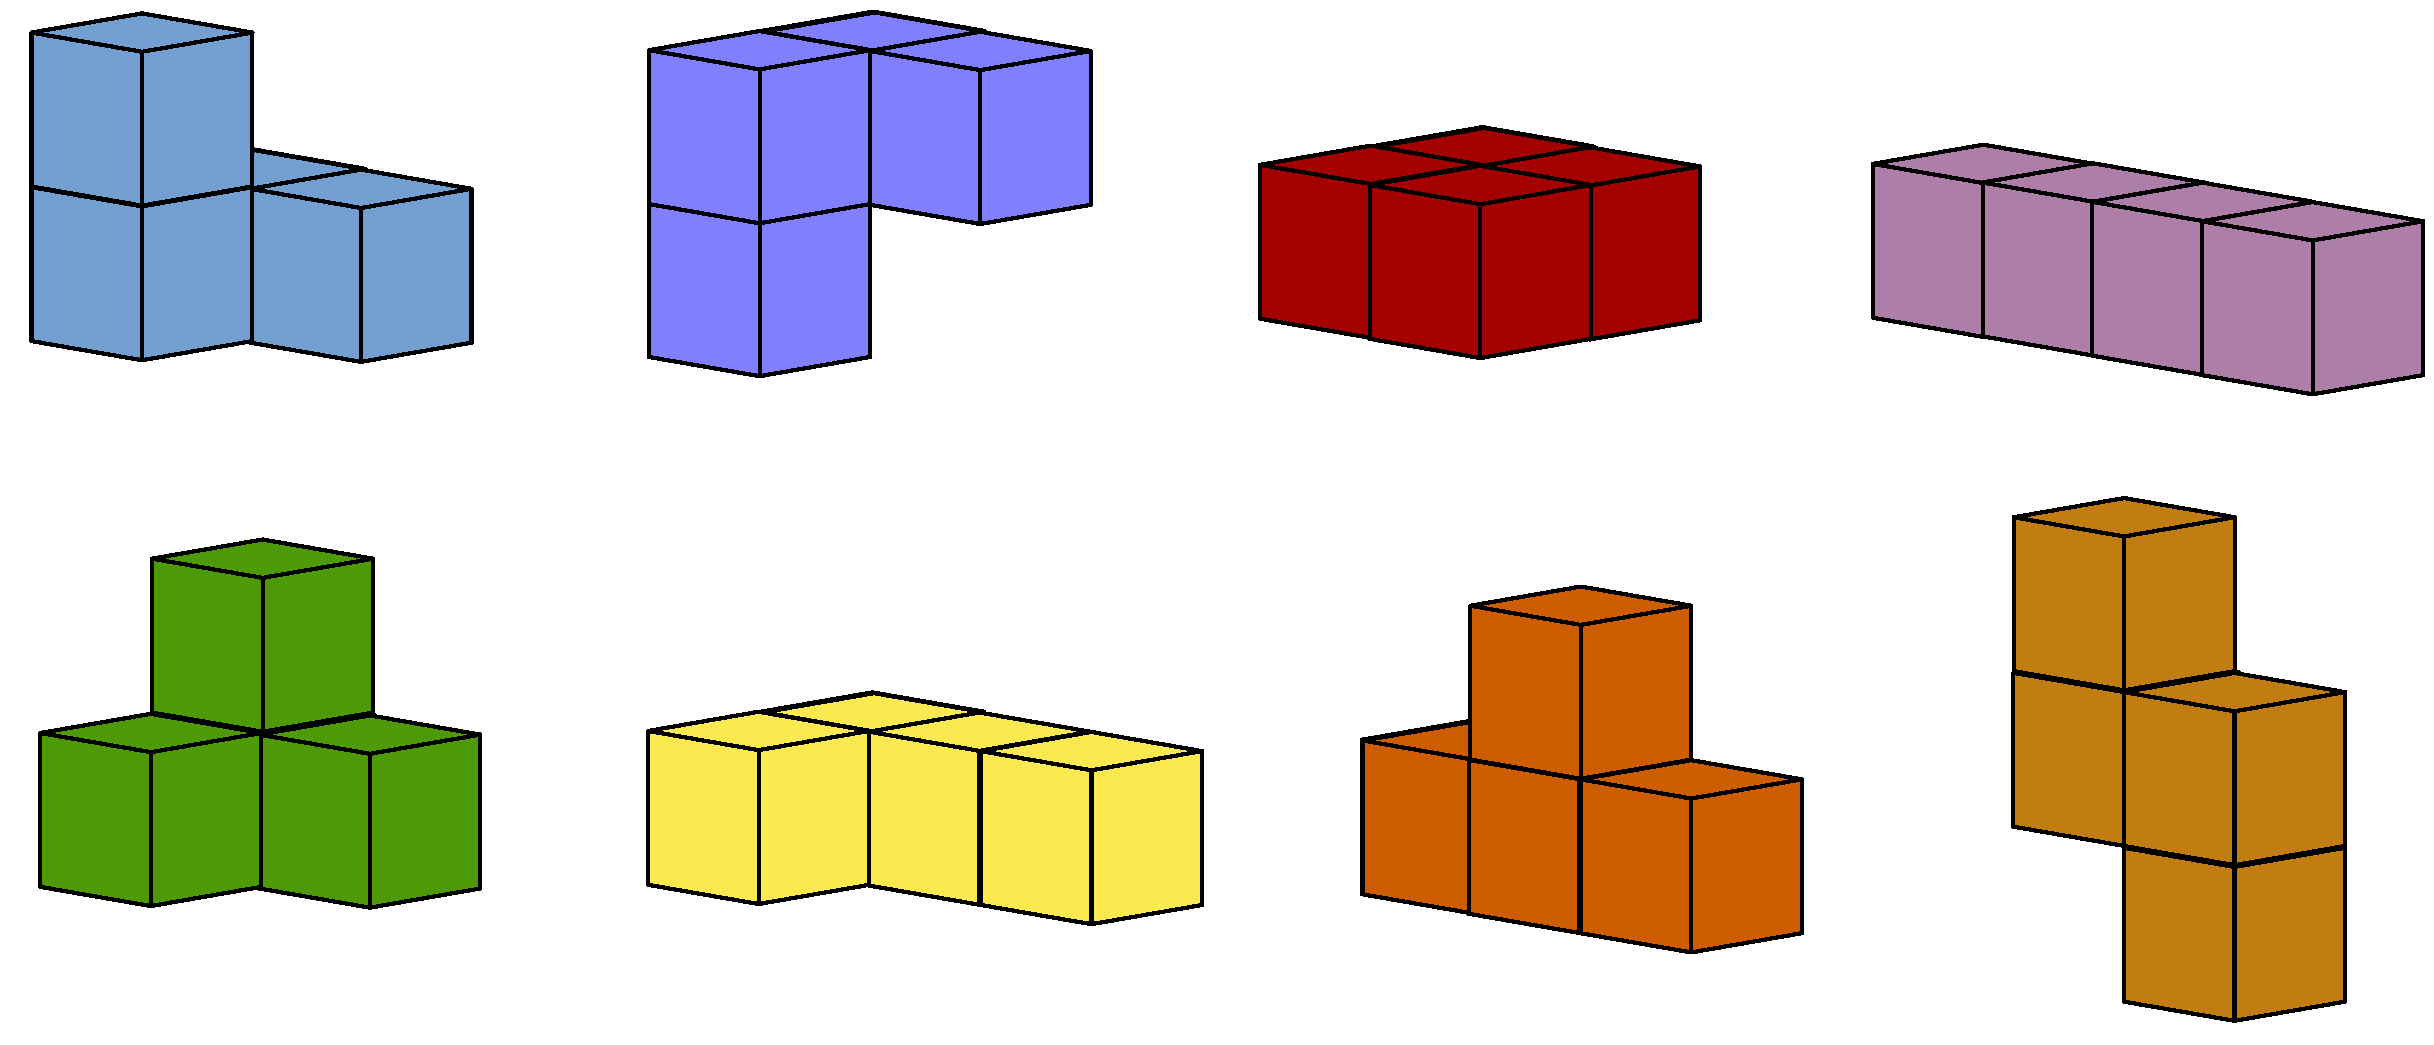
\includegraphics[width=0.8\textwidth]{figures/tetris-pieces.pdf}
%     \caption{The 8 different 3D Tetris pieces, with the first two pieces being mirror images of each other.} 
%     \label{fig:tetris-pieces}
% \end{figure}

% Note that the first two pieces are non-superimposable mirror reflections of each other; they are \emph{chiral}.

% We use a simple message-passing neural network, described in Algorithm \ref{alg:mpnn}, using either the Gaunt and Clebsch-Gordan tensor products. The form of our network is quite popular, and first introduced by \citep{nequip}.

% Given a randomly oriented 3D structure, the network needs to predict which of the 8 tetris pieces it corresponds to.

% The pieces are normalized such that the side length of each cube is $1$. When represented as a graph, the center of each cube is a node.
% We instantiate the network with $d_\text{max} = 1.1$ so that the centers are connected only to its immediately adjacent centers. 
% The networks finally outputs $\x = 7\times0e + 1\times0o$ irreps. (As a reminder, $0e$ are scalars and $0o$ are pseudoscalars). The logits and predicted probabilities are then computed by:
% \begin{align*}
%     l_0 &= \x^{(0o)} \times \x^{(0e)_0} \\ 
%     l_1 &= -\x^{(0o)} \times \x^{(0e)_0} \\
%     l_i &= \x^{(0e)_{i}} \quad \text{ for } i \geq 2  \\
%     p_i &= \textrm{softmax}(l_i)
% \end{align*}
% It is clear that defining the logits in this manner preserves the rotational and reflection symmetries. The predictions are clearly invariant under rotations (as they are $\ell = 0$ irreps), and under reflections: $\x^{(0o)} \to -\x^{(0o)}$ but $\x^{(0e)_i} \to \x^{(0e)_i}$.

% We set the number of message-passing steps $T$ to be $3$, to allow the interactions $1o \otimes 1o \to 1e$ and then $1e \otimes 1o \to 0o$, so that the pseudoscalar can be created. The degree of spherical harmonics is kept as $\ell = 4$. The irreps of the hidden layers are restricted to some cutoff $L$, which is varied from $1$ to $4$ to vary the expressivity of the network.
% The network is trained with the Adam optimizer with learning rate $0.01$ to minimize the standard cross-entropy loss.

% \begin{figure}
%     \centering
%     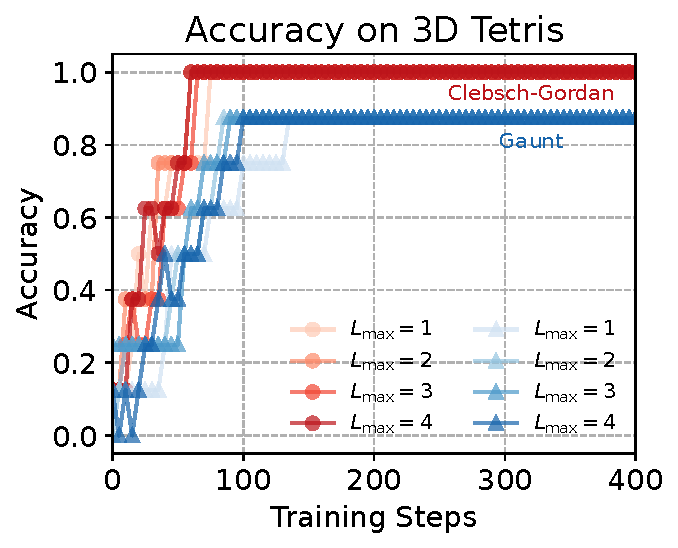
\includegraphics[width=0.6\textwidth]{figures/tetris-results.pdf}
%     \caption{Training curves of networks trained with different tensor products on the 3D Tetris task. The maximum $L$ is varied from $1$ to $4$. All of the Clebsch-Gordan networks attain $100\%$ accuracy while none of the Gaunt networks do.} 
%     \label{fig:tetris-results}
% \end{figure}

% \begin{algorithm}
% \caption{Operation of our Message Passing Neural Network}
% \label{alg:mpnn}
% \begin{algorithmic}
% \Require Graph $G$, Message Passing Iterations $T$, Cutoff $d_{\text{max}}$, Spherical Harmonic Degree $\ell$, Tensor Product $\otimes$
% \State Compute neighbor lists for each node in $G$:
% $$(u, v) \in E \iff \norm{\mathbf{r}_u - \mathbf{r}_v} \leq d_{\text{max}}$$
% \For{$v \in V$}:
% \Let{$h_v^{(0)}$}{$[1]$}
% \EndFor
% \For{$t = 1, 2, \ldots, T$}:
% \For{$v \in V$}:
% \Let{$h_v^{(t)}$}{$\textsc{Linear}(h_v^{(t - 1)}) + \textsc{Linear}(\frac{1}{C}\sum_{u \in \gN(v)} h_u^{(t - 1)} \otimes Y_\ell(\mathbf{r}_u - \mathbf{r}_v))$}

% \EndFor
% \EndFor
% \State \Return $\{h_v^{(T)}\}_{v \in V}$  
% \end{algorithmic}
% \end{algorithm}

% As shown in \autoref{fig:tetris-results}, the  network is very easily able to solve this task with the Clebsch-Gordan tensor product, but the same network parametrized with the Gaunt tensor product is unable to distinguish between the two chiral pieces. Adding more channels or incorporating the pseudo-spherical harmonics (which have the opposite parity of the spherical harmonics under reflection) did not help. The fundamental failure is the inability to create the $1e$ term via $1o \otimes 1o \to 1e$ because this is the cross product, ie an antisymmetric operation. Indeed, there is no way to create a pseudoscalar using the Gaunt tensor product in this setting.

